\subsubsection{Introduktion}

Begge klasser i \gls{KA} Business Logic Layer anvender ObservableCollection<T>~\cite{ObsCol}. ObservableCollection<T> bliver benyttet så begge klasser, kan behandles som en list<> af deres model objekter.\\
ShoppingList anvender desuden RelayCommand~\cite{RelayC} for at denne klasse kan implementeres efter MVVM~\cite{MVVM} pattern, med commands som kan bindes til \gls{GUI} knapper. 

\begin{figure}[H]
	\centering
	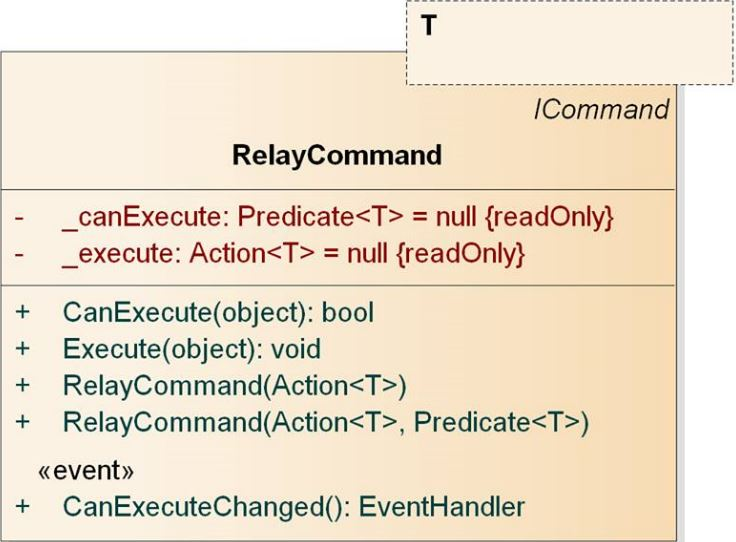
\includegraphics[width=60mm]{Systemdesign/Frontend/BLL/Pics/Relay}
	\caption{RelayCommand}
	\label{fig:RelayCmdKasse}
\end{figure}